\chapter{The Tangle}
This chapter covers the fundamental building blocks of the directed acyclic graph (DAG) architecture of IOTA called Tangle \cite{the-tangle}.
\section{Participation in the network}
The tangle does not know the discrepancy of validating nodes (miners) and issuing nodes in a sense that Bitcoin does. Every node in the network can issue and validate transactions. A new transaction is  
what motivates nodes to validate and propagate transactions. Each node calculates statistics about the activity of its neighbors. If a neighbor appears to be lazy, it can be dropped. For this reason, a node in the network is incentivized to participate in the network, even at times when it does not issue transactions. 

\section{Transactions}
As there are no miners in the network, transactions are being validated by other nodes that issue transactions themselves. In order to create a new transaction on the network, a node does the following steps:
\begin{enumerate}
    \item The node chooses two unconfirmed transactions according to an Monte Carlo Walk algorithm which will be described in more detail in Section \ref{tip-selection}.
    \item The node is responsible for checking the validity of these two transactions. Conflicting transactions are ignored.
    \item A node has to perform a cryptographic puzzle in order to make the new transaction valid. Similar to the Proof of Work (PoW) mechanism in Bitcoin, this puzzle is solved with computational resources. The puzzle is defined by finding a nonce such that the hash of this number concatenated with some data from the approved transactions results in a number smaller than some predefined constant. This puzzle is necessary in order to prevent several attack scenarios which will be discussed in Section \ref{attacks}.
\end{enumerate}

The next section describes the basic concepts of the tangle. For all figures, a box resembles a transaction and the directed edge between nodes illustrates the approval of a transactions. In order to understand the approval algorithm, the following five parameters are defined for every transaction.
\begin{description}
    \item[weight] The weight of a transaction is defined by the amount of work that the issuing node has invested in to this transaction. The weight of a transaction resembles its importance. This measurement helps to prevent spamming and other attacks since no node can create an abundance of transactions with meaningful weights within a short period of time. 
    \item[cumulative weight] The cumulative weight of a transaction is calculated by the weight of the transaction itself plus the sum of all transactions that directly or indirectly approve this transaction. Figure \ref{fig:cumulative-weight} shows how the weight and the cumulative weight change after the new transaction \textit{X} is added, the smaller number denotes the weight of a node and the bold number represents cumulative weight of a transaction.\par
        \begin{minipage}{\linewidth}
            \centering
            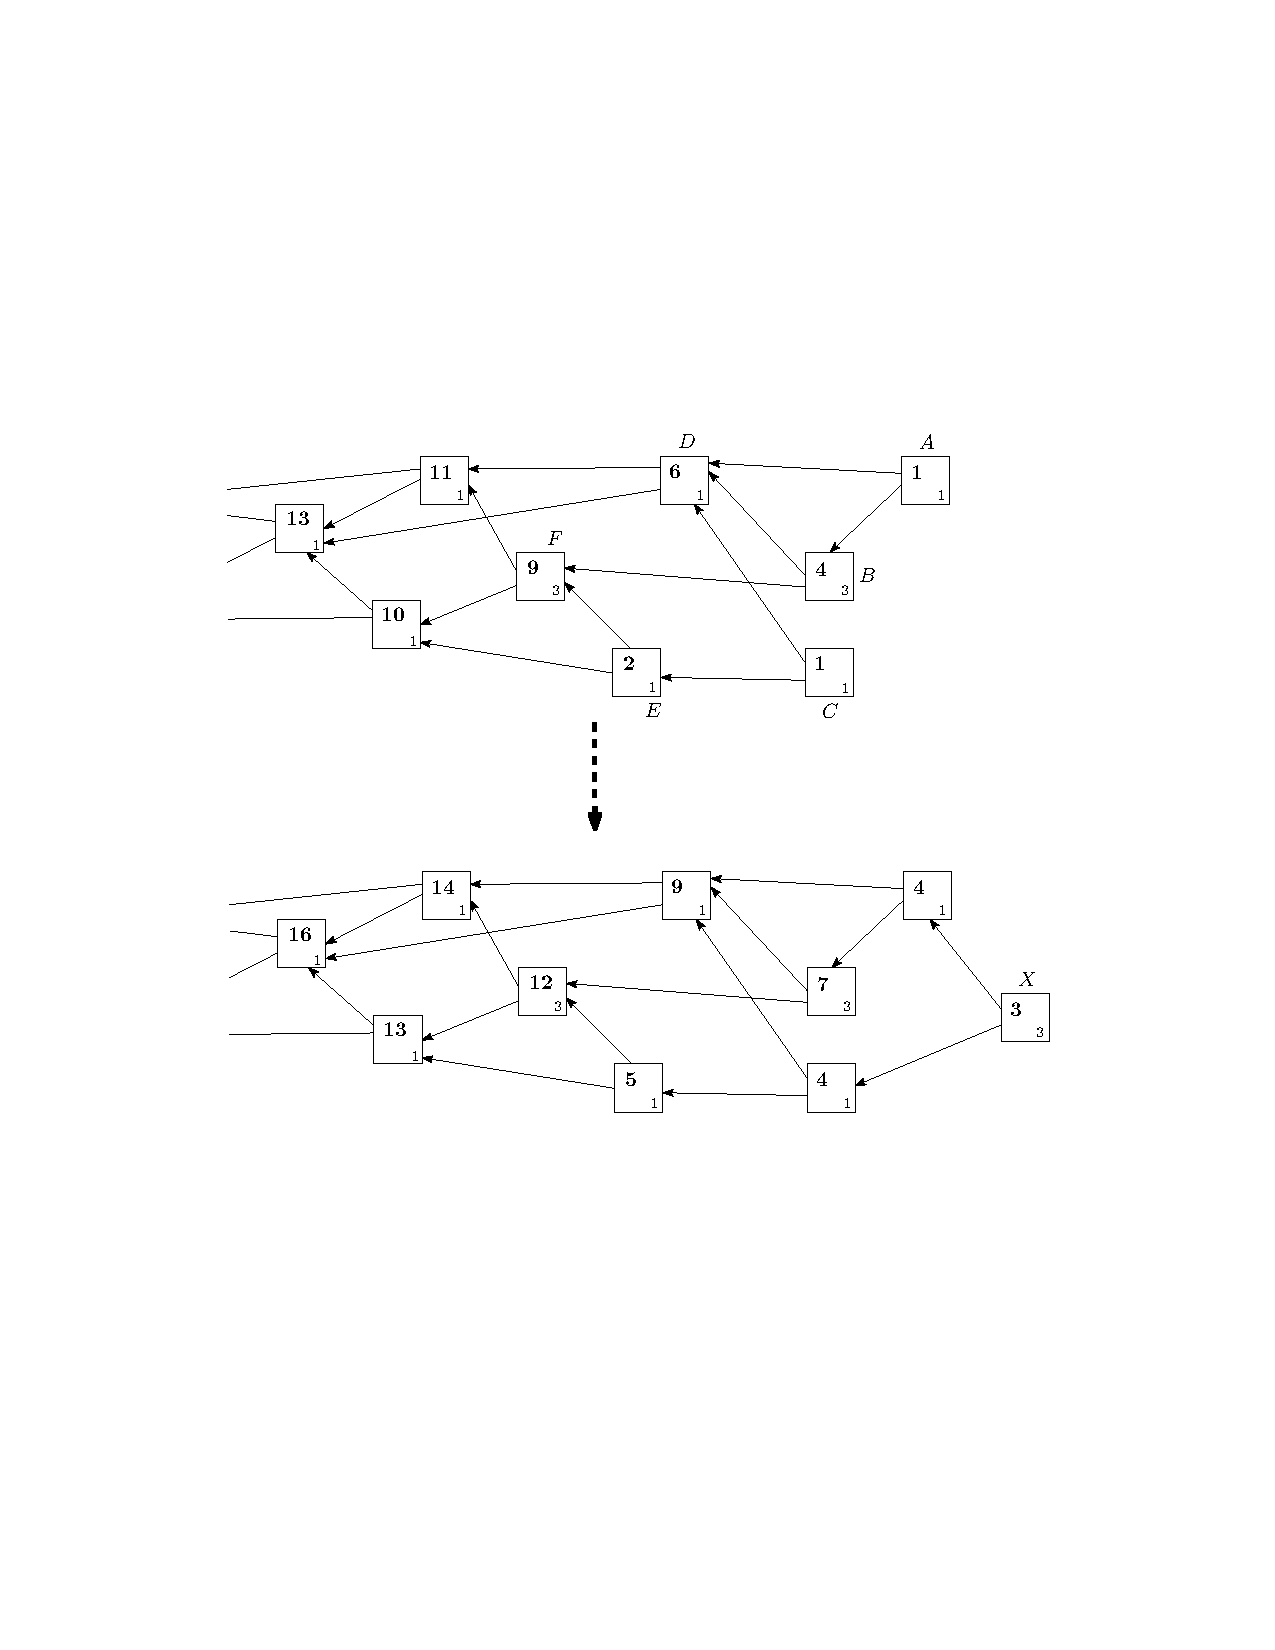
\includegraphics[width=10cm]{images/cummulative_weight.pdf}
            \captionof{figure}{Cumulative Weight \cite{the-tangle}}
            \label{fig:cumulative-weight}
        \end{minipage}
    \item[height] The height of a transaction is the length of the longest oriented path to the genesis transaction. In Figure \ref{fig:height-depth-score}, transaction \textit{G} has a height of 1 due to the blue edge.
    \item[depth] The depth of a transaction is the length of the longest reverse oriented path to some tip. In Figure \ref{fig:height-depth-score}, transaction \textit{G} has a depth of 4 due to the red approvals from newer transactions \textit{F, D, B} and \textit{A}.
    \item[score] The score of a transaction is the sum of weights of all transactions that are approved by this transaction plus its own weight. The scores for transactions \textit{A} and \textit{C} are shown with the circled number in Figure \ref{fig:height-depth-score}.\par
        \begin{minipage}{\linewidth}
            \centering
            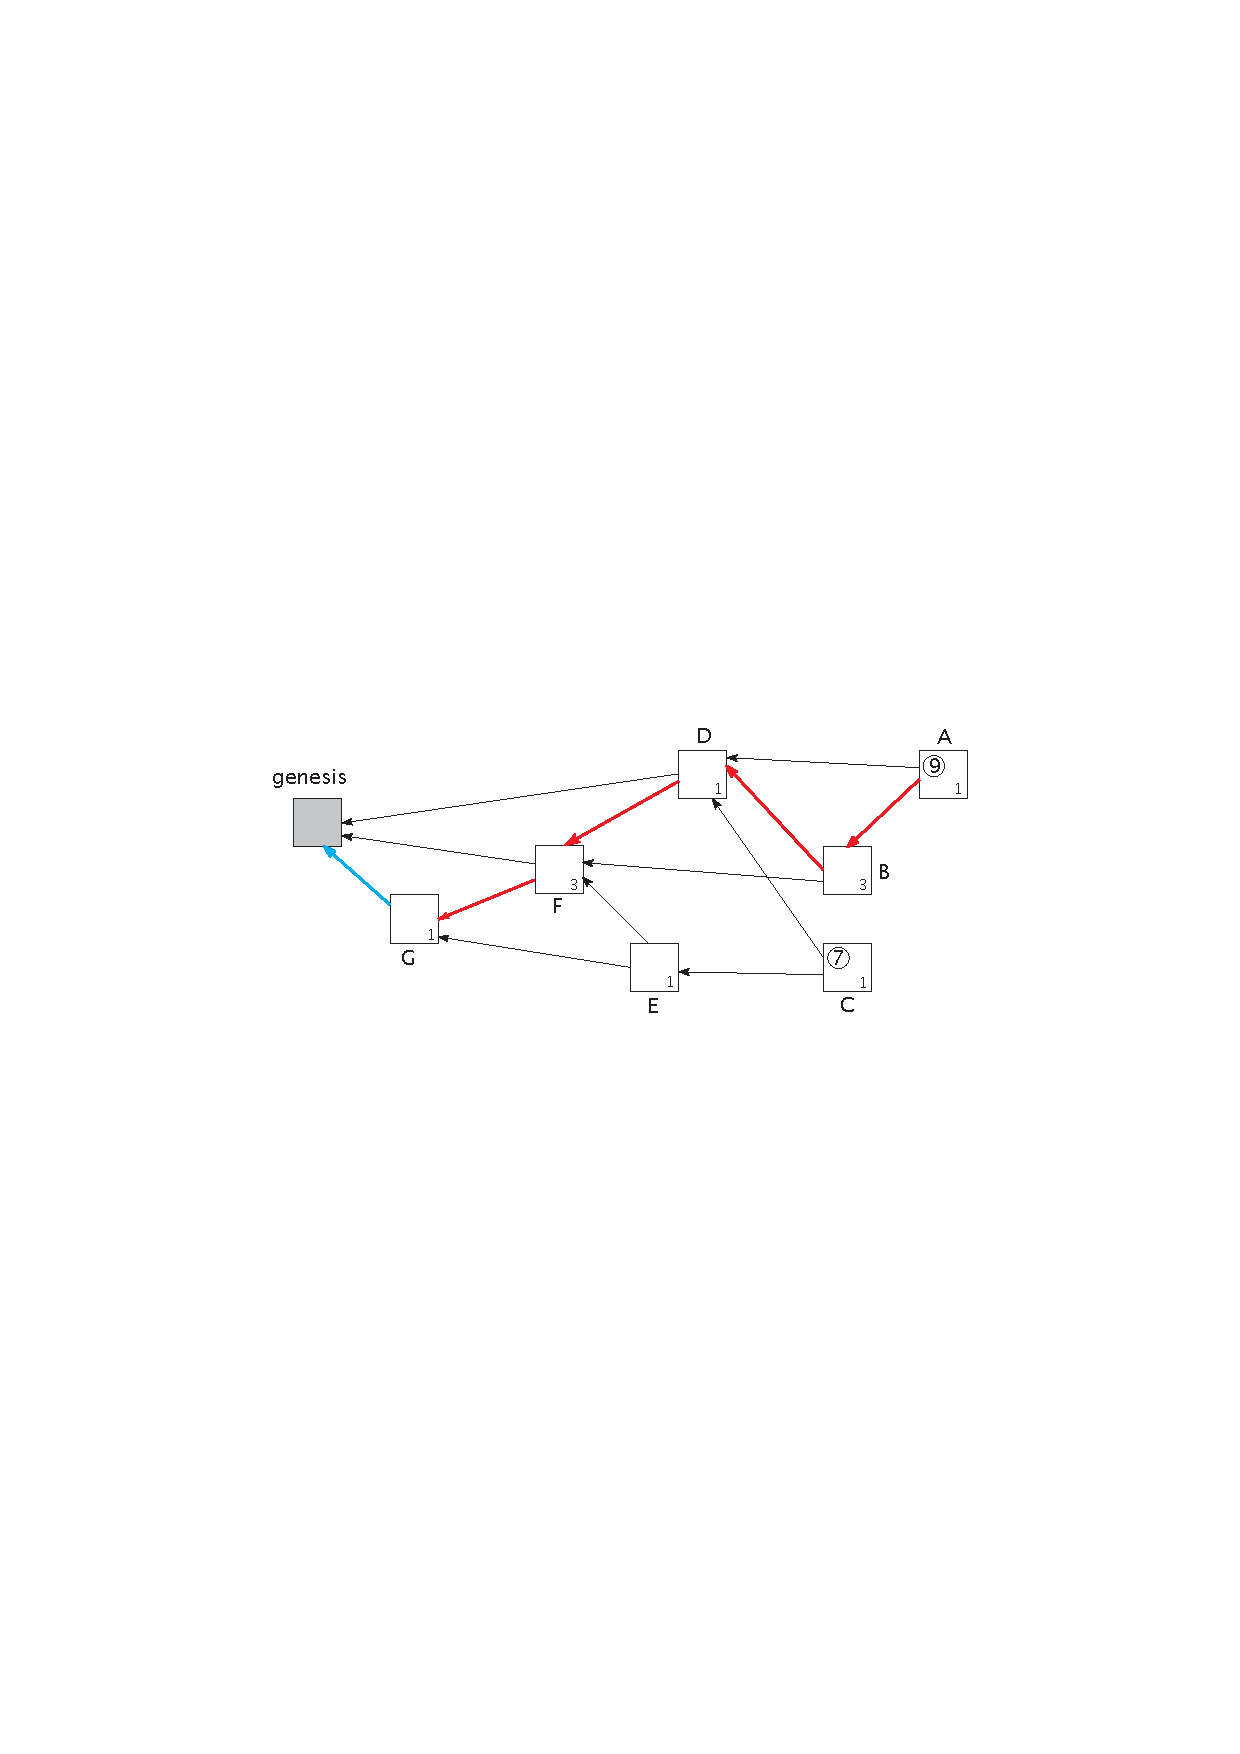
\includegraphics[width=12cm]{images/height-depth-score.pdf}
            \captionof{figure}{Height, Depth and Score \cite{the-tangle}}
            \label{fig:height-depth-score}
        \end{minipage}
\end{description}

These parameters will play an important role when discussing tip selection in Section \ref{tip-selection} and attack scenarios \ref{attacks}.

\section{Tip Selection}\label{tip-selection}
Unapproved transactions are called tips. This section covers the reasons why the process of selecting a tip is important for the network.
In order to discuss the tip selection algorithm, a simulation of the DAG architecture is characterized by the following two parameters. 


\begin{description}
    \item[Transaction rate $\gamma$] Transactions do not arrive evenly throughout time. To model such behaviour, a mathematical object called Poisson point process is used. The arrival rate of transactions is specified by the parameter $\gamma$. The higher $\gamma$ is set in the simulation, the more transactions arrive within one time-unit. If $\gamma$ is set to a really small number, the graph grows in the form of a linked list as there is always just one tip to be approved by a new transaction. Figure \ref{fig:simulation} shows a simulation, where $\gamma=5$. The tips are drawn as grey boxes.
    \item[Delay $h$] As new transactions must perform computational work for spam prevention and this computation is based on the selected tip of that transactions, there is a delay between choosing the tips and publishing the transaction. This delay is defined by the parameter $h$. For a device with less computational power, $h$ will be larger than for computers with higher processing power. The simulation in Figure \ref{fig:simulation} assumes that $d=1$ for every device that adds a new transaction. Thus, for example the node issuing transaction 5 did not know about the transactions 1-4 when he started with the PoW computation for transaction 5. The time difference to transactions 1-4 is less than $d$. 
\end{description}

\begin{figure}[H]
    \centering
    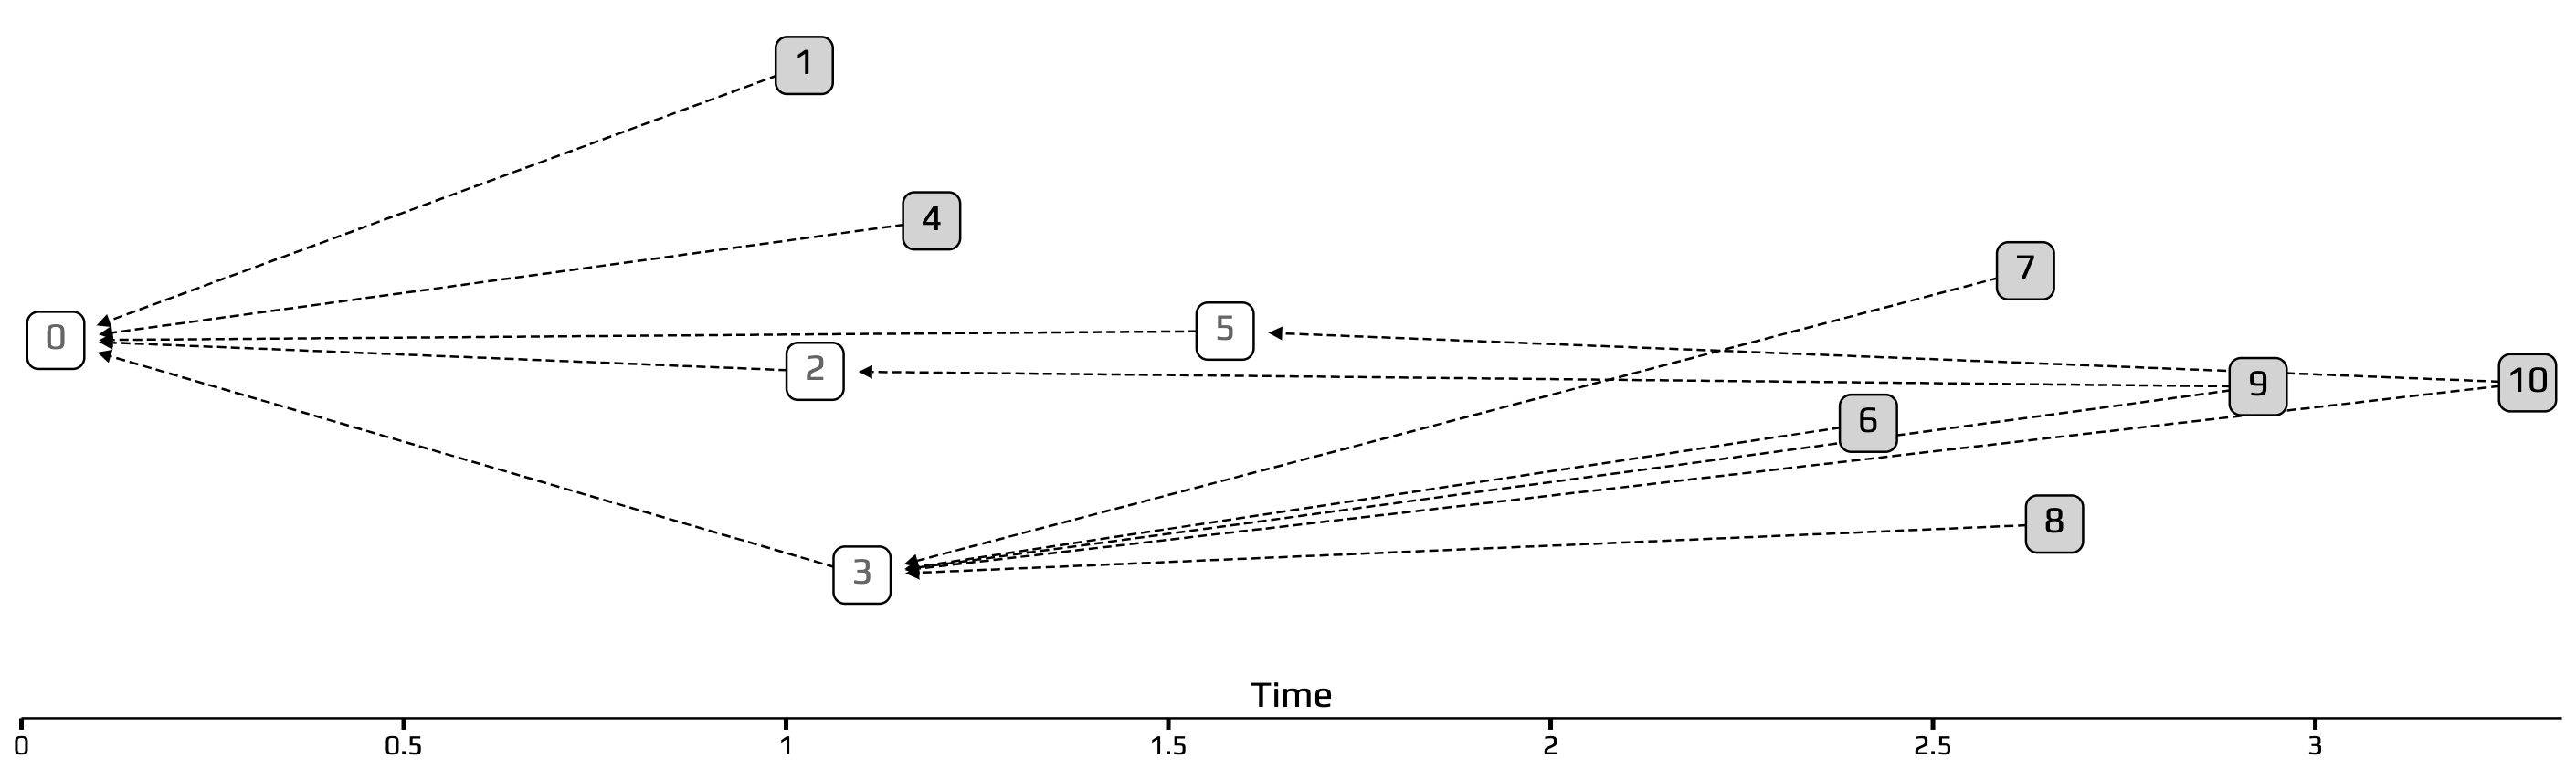
\includegraphics[width=1.0\textwidth]{images/simulation.png}
    \caption{Simulation with $\gamma=5$ and $d=1$  \cite{the-tangle-part-3}}
    \label{fig:simulation}
\end{figure}


There is a possibility that one or both of the validated transactions might no longer be a tip at the time of broadcasting the new transaction. Thus, the tangle must also accept transactions that approve already verified transactions. However, the tip selection algorithm must avoid these \textit{lazy tips} which point to older transactions. Confirming old transaction is unwanted since it increases the branching factor of the graph and thus, it increases the number of tips. Furthermore, \textit{lazy} nodes do not help the network to grow since no unapproved transactions are confirmed. In Figure \ref{fig:lazy-tip}, transaction 14 is added to the network by a lazy node. 


\begin{figure}[H]
    \centering
    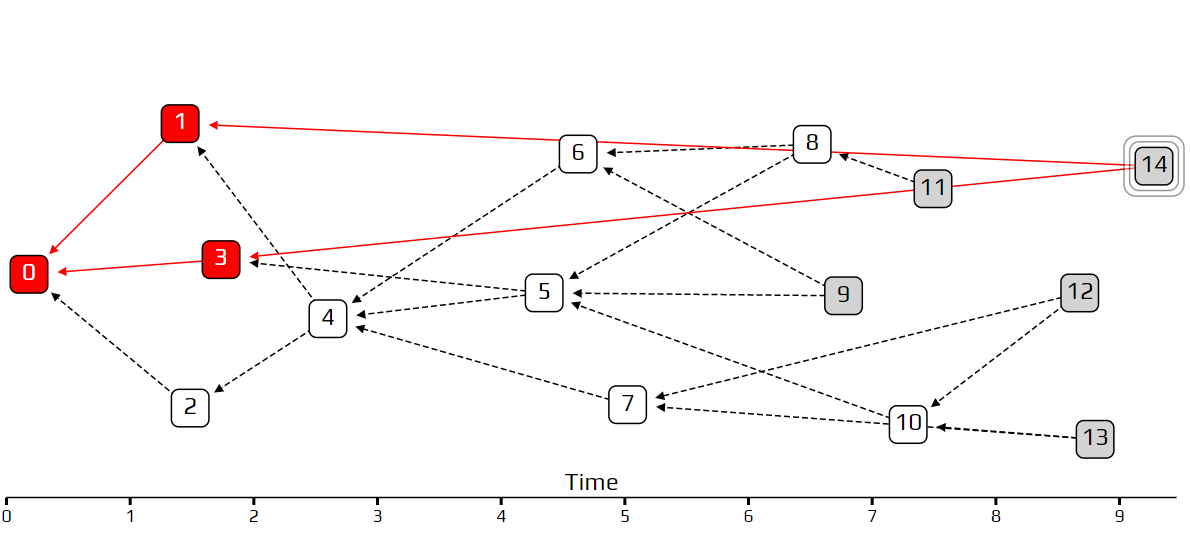
\includegraphics[width=1.0\textwidth]{images/lazy-tip.png}
    \caption{Lazy Tip \cite{the-tangle-part-3}}
    \label{fig:lazy-tip}
\end{figure}

For finding a tip, a node must walk from the genesis until it reaches an unconfirmed transaction. The node has to choose between multiple possible paths. If the node chooses the path solely based on the branching factor, transactions added by lazy nodes would be selected with the same probability as any other transaction. Thus, the random walk algorithm must be less biased towards lazy transactions. 
This is achieved by favoring transactions that have a higher cumulative weight. The bias factor is defined with the parameter $\alpha$. Setting $\alpha$ to a high value results in many unconfirmed transactions since most approvers choose the same path to the tip. These unconfirmed transactions are left behind and will never be accepted. Thus, determining an ideal value for $\alpha$ is crucial for the usability of the network and depends on the transaction arrival rate, the PoW delay of different devices in the network, network delay and the number of tips. 

The method of setting a rule on how to find a path towards a tip is called a Markov Chain Monte Carlo technique (MCMC) \cite{mcmc}. In a Markov chain, each step enforces a rule which is defined in advanced and does not depend on the previous step. In the example of the Tangle, each step is a node in the graph and the rules are the probabilities of the available paths depending on the cumulative weights.

\section{Transaction Validation}\label{transaction-validation}
The transaction validation process is similar to Bitcoin's unspent transaction output (UTXO) model. An unspent transaction output is the output of a transaction that a user receives and is able to spend in the future. Thus, the validating node must check all previously made transactions of the sender address in order to verify a transaction. The smallest unit of the underlying currency is also called IOTA. All IOTA are minted in the genesis transaction and therefore, every IOTA can be traced back to genesis block. 

Transactions cannot be seen as valid as soon as one approver has referenced it. Thus, a new parameter is introduced called confirmation confidence. The confirmation confidence for a transaction $X$ can be calculated in the following way.

\begin{enumerate}
    \item The tip selection algorithm is run 100 times.
    \item The number of tips that approve transaction $X$ is counted.
    \item Every tip is weighted by the likelihood that it will be accepted in the future.
    \item The confirmation confidence of transaction $X$ is the fraction of approving transactions.
\end{enumerate}

It is assumed that transactions are issued by a large number of independent entities, so the process of incoming transactions can be modeled Poisson point process \cite{the-tangle}. $\lambda$ denotes the rate of the Poisson process and it is assumed that it remains constant in time. At some point in time, every new transaction will approve transaction $X$ since all tips include a path to transaction $X$. Thus, after the adoption period, the cumulative weight will grow linearly with $\lambda * w$ where $w$ is the average weight of a transaction.

\begin{figure}[H]
    \centering
    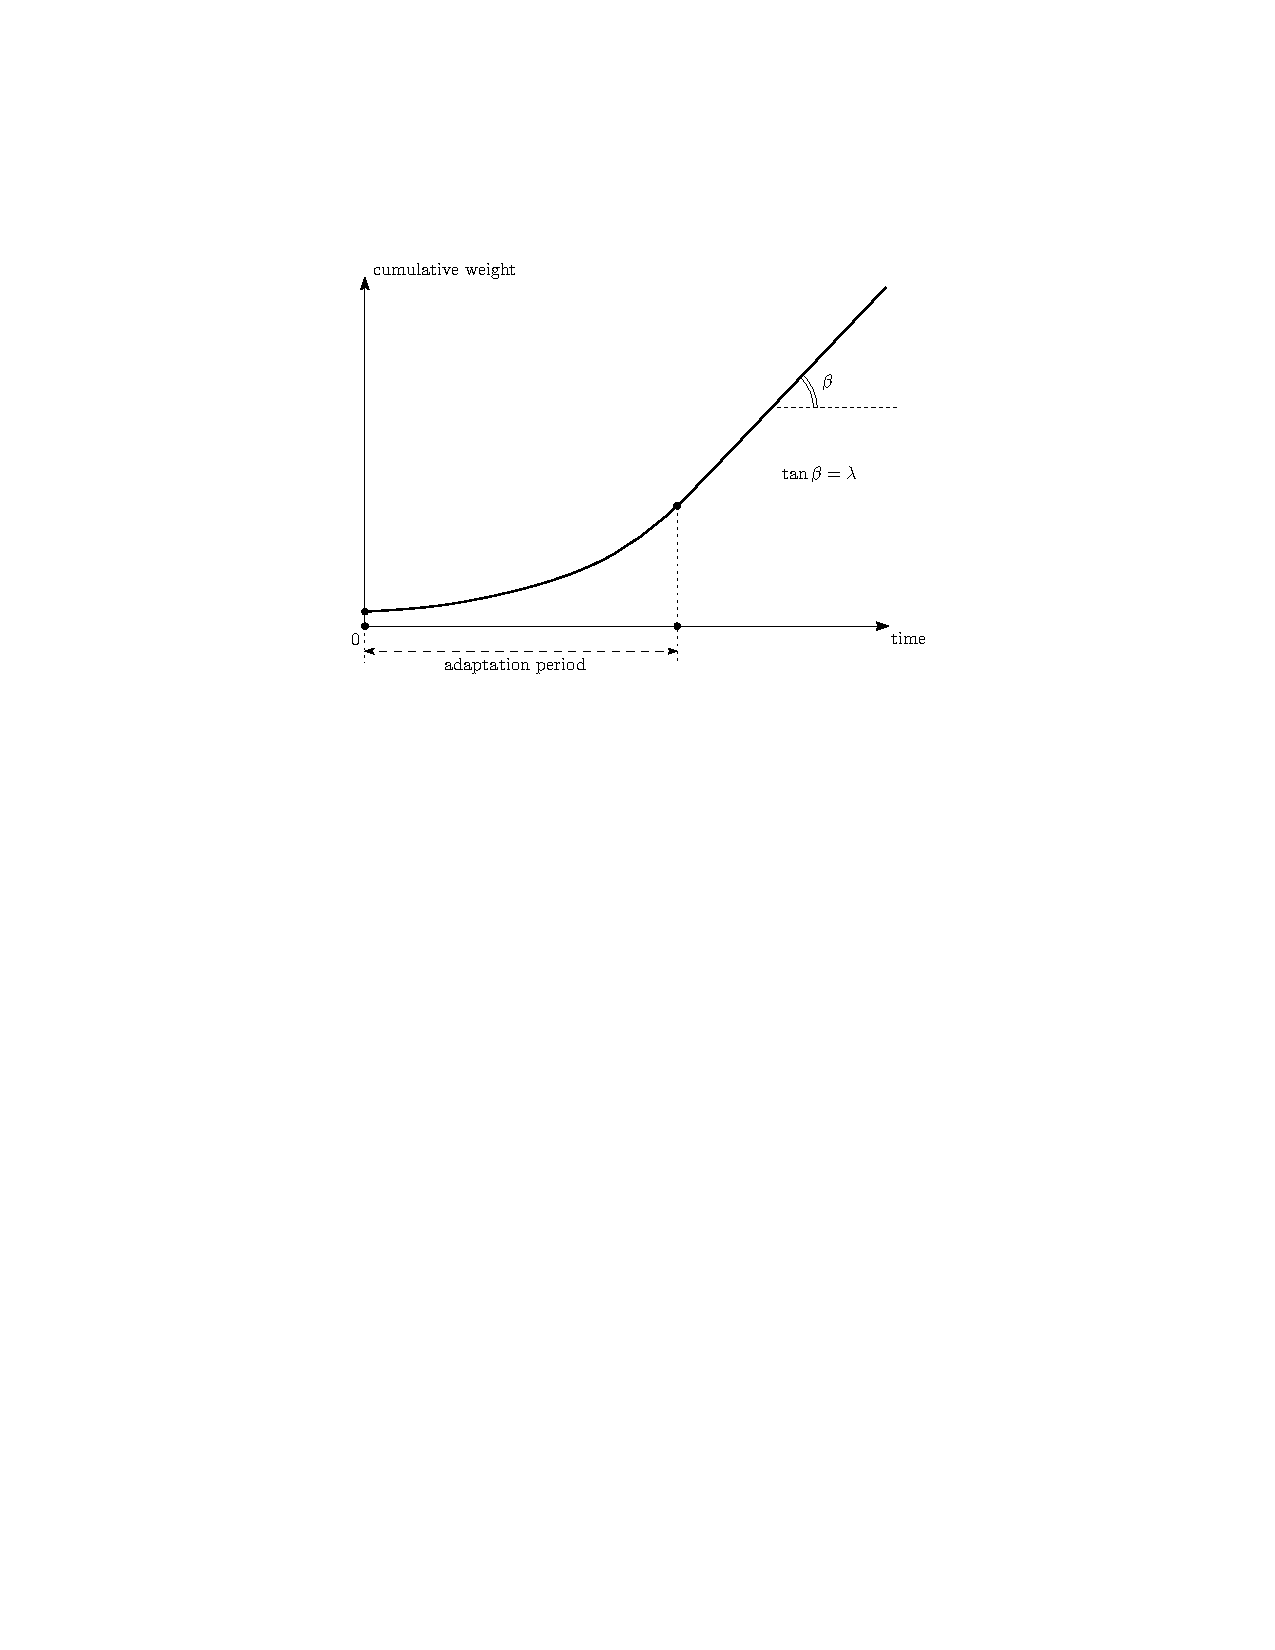
\includegraphics[width=8cm]{images/confirmation-confidence.pdf}
    \caption{Confirmation Confidence and Cumulative Weight Growth \cite{the-tangle}}
    \label{fig:confirmation-confidence}
\end{figure}

In Figure \ref{fig:confirmation-confidence-tangle}, transactions with confirmation confidence of more than 0.95 have a thick border. Almost any new honest transaction that is added to this tangle will confirm these transactions (except lazy nodes with lazy tip selection). In the shown example, transaction 9 confirms all the red transactions and is confirmed by the blue transactions. There are four tips in the shown simulation - 6, 10, 11 and 12. The confirmation confidence of transaction 9 is 0.94 due to the fact that transactions 10, 11 and 12 have more importance than 6.
Transaction 4 has confirmation confidence of 1 since all tips have a path to transaction 4 and therefore, there is no transaction in the network that does not confirm this transaction.

\begin{figure}[H]
    \centering
    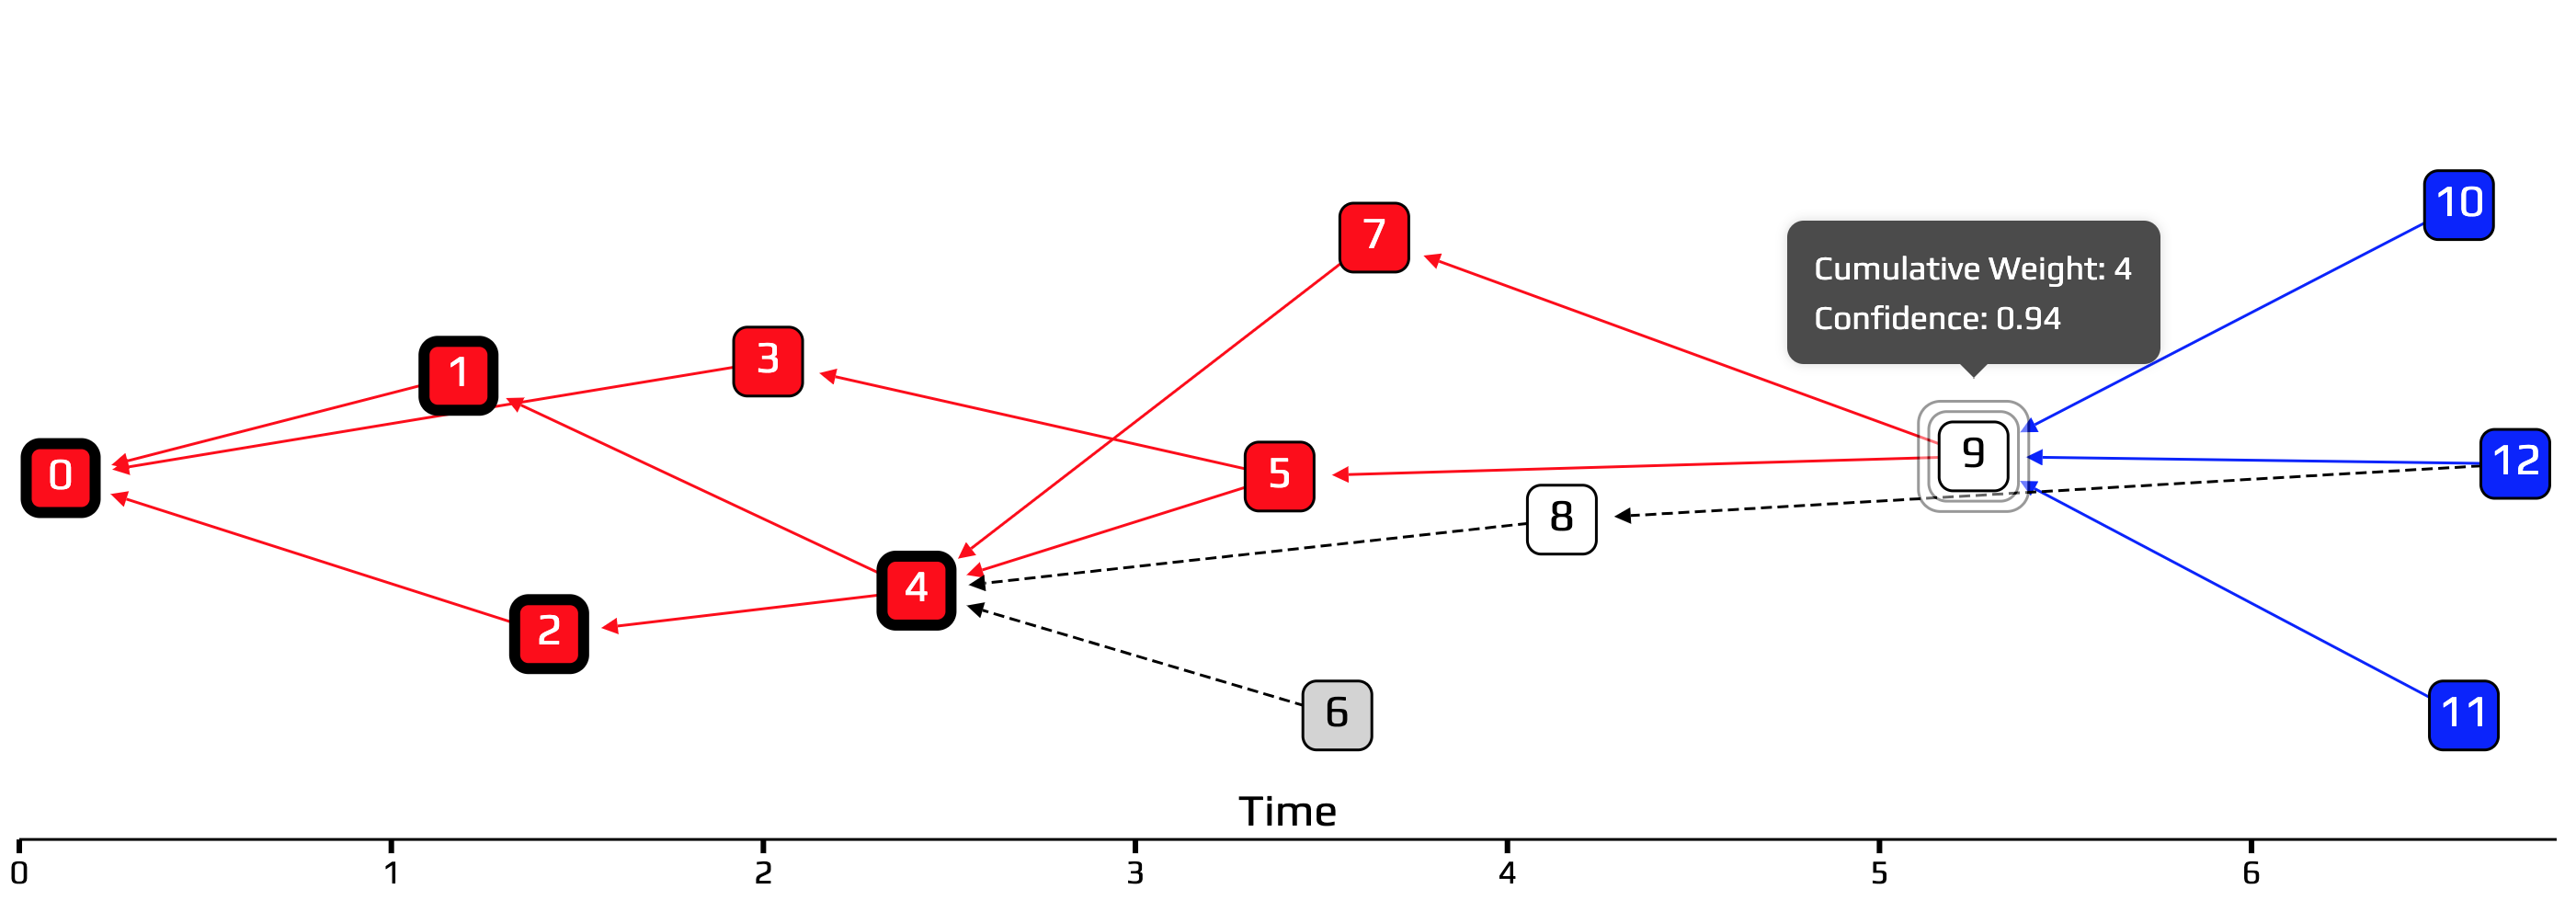
\includegraphics[width=1.0\textwidth]{images/confirmation-confidence-tangle.png}
    \caption{Graph Representation of the Confirmation Confidence}
    \label{fig:confirmation-confidence-tangle}
\end{figure}

\section{Attacks}\label{attacks}
This section covers some of the possible attack scenarios and how the Tangle can still maintain consensus among honest users.

\subsection{Double Spend}
A double spend situation occurs when a user tries to exceed his account balance by issuing two or more conflicting transactions. Figure \ref{fig:double-spend} illustrates such a scenario. A box represents a transaction. The dashed box inside represents the current state in the graph but is not part of an actual transaction. In this simulation, Alice owns only 15 IOTA but issues two transactions with 10 IOTA each. Bob cannot approve both of Alice's transactions as they result in a negative account balance.

\begin{figure}[H]
    \centering
    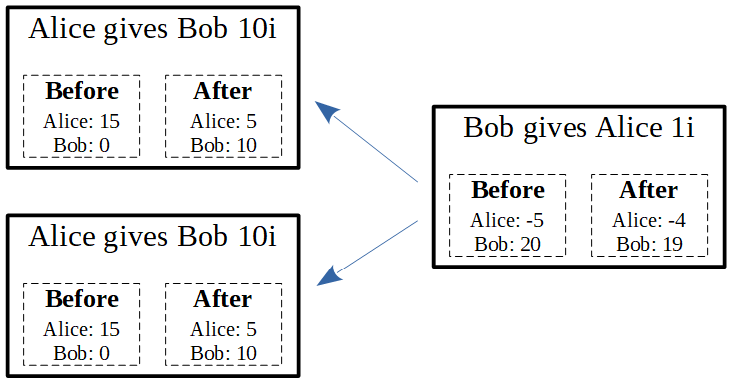
\includegraphics[width=8cm]{images/double-spend.png}
    \caption{Double Spend Attack \cite{the-tangle-part-5}}
    \label{fig:double-spend}
\end{figure}

The solution to this problematic situation is the weighted random walk discussed in Section \ref{tip-selection}. One of the two transactions will become heavier and the lighter one will be abandoned. This implies that a confirmed transaction cannot be considered as valid as soon as it has been approved for the first time. 

Confirmation confidence is introduced in Section \ref{transaction-validation} and provides a measurement of what percentage the network has directly or indirectly approved a transaction. 


\subsection{Large Weight Attack}
The large weight attack has the same intent as the double spend but actively tries to invalidate a transaction with high confirmation confidence. This can be achieved by a malicious user as follows.

\begin{enumerate}
    \item A transaction is created and broadcasted that is intended to revert.
    \item The malicious user waits until the receiver believes the transaction has a high enough confirmation rate. The merchant ships the product/service.
    \item The attacker uses its computational power and issues a double-spending transaction with a large weight followed by many more transactions. This transaction does not approve the first transaction and thus they compete with each other for finality.
    \item The bad actor hopes that the dishonest subtangle gains more cumulative weight than the honest subtangle.
\end{enumerate}

\begin{figure}[H]
    \centering
    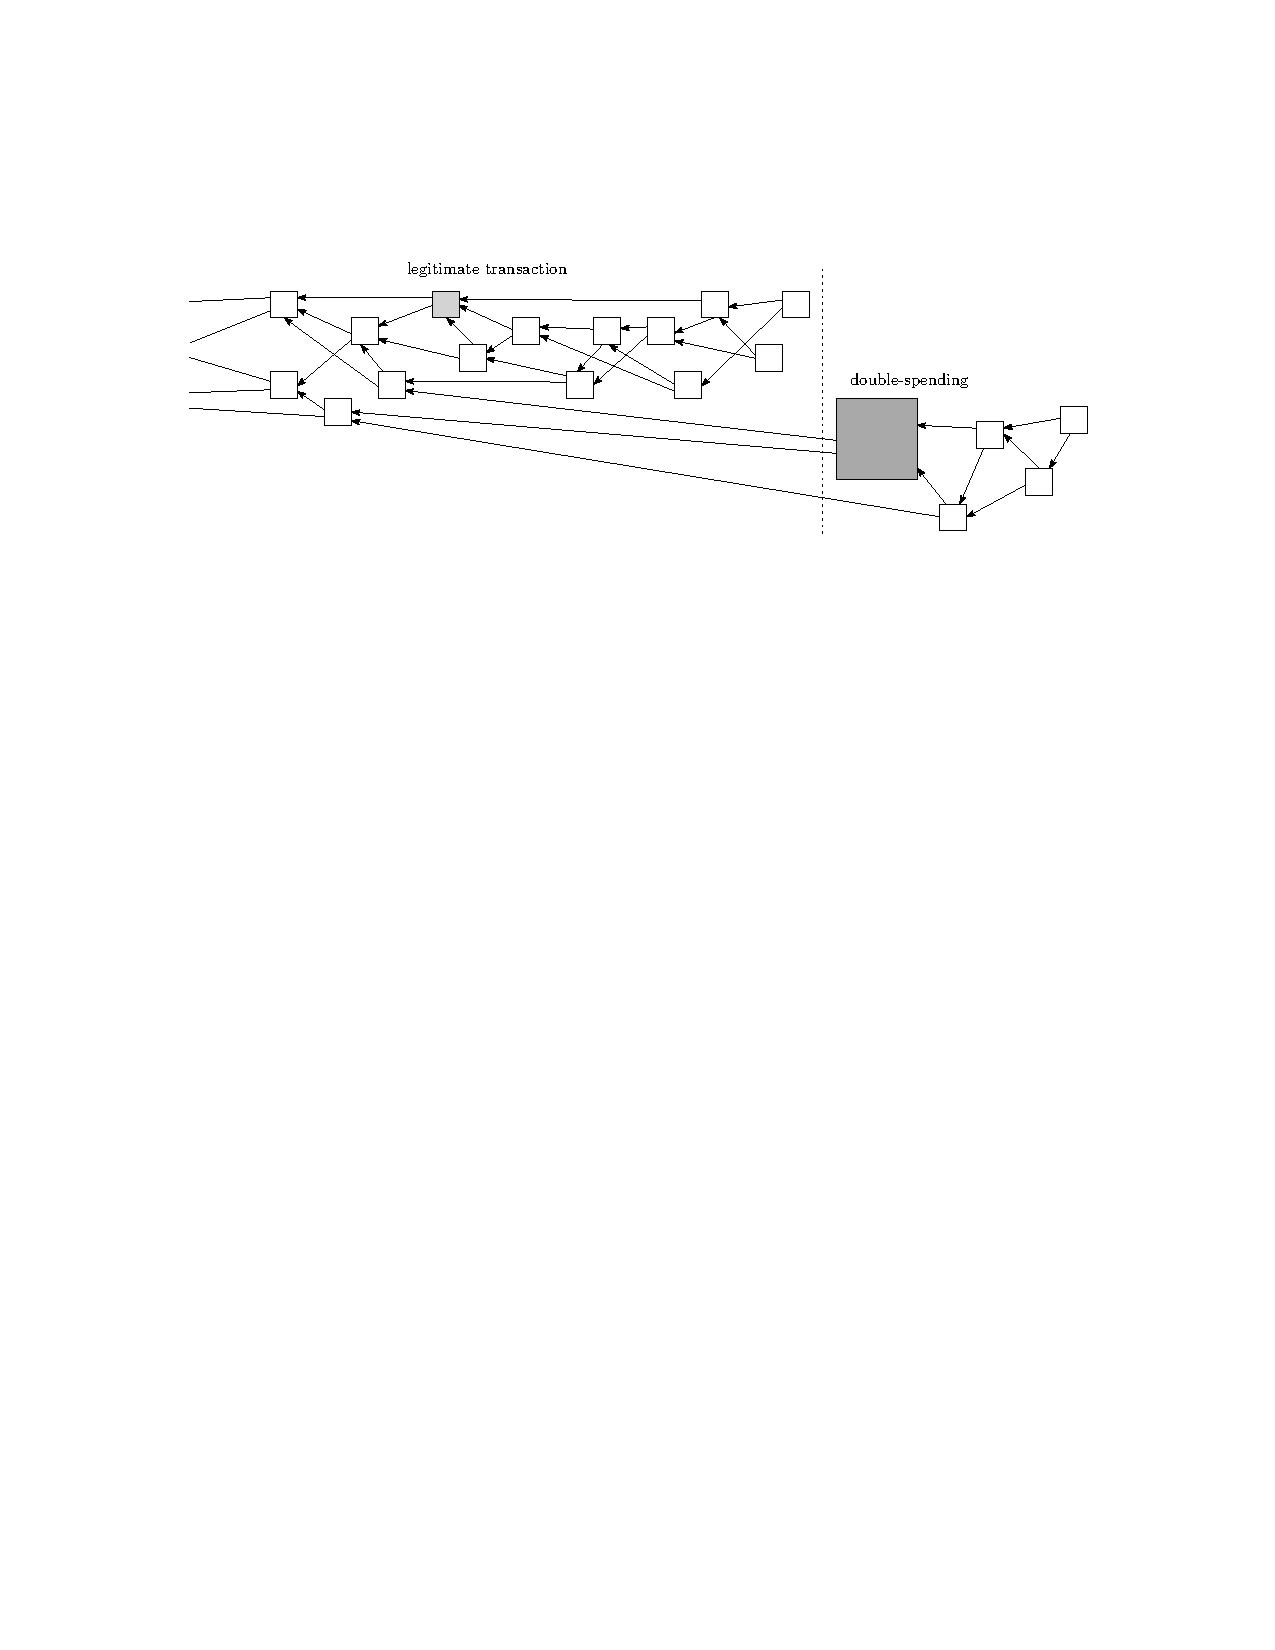
\includegraphics[width=12cm]{images/large-weight-attack.pdf}
    \caption{Large Weight Attack \cite{the-tangle}}
    \label{fig:large-weight-attack}
\end{figure}

This attack can only be carried out if the attacker has more computing power than all the nodes that actively issue new transactions. In a well-established network with many nodes issuing transactions, this is less of an issue. In the early stages, however, there are not enough transactions passing through the network in order to be safe from such an attack. Due to this reason, the IOTA foundation has put a coordinator in place which is discussed in more detail in Section ?.

\subsection{Parasite Chain Attack}
The parasite chain attack also tries to convince the network to abandon a previously confirmed transaction by biasing the tip selection algorithm.The attack works as follows:
\begin{enumerate}
    \item The attacker creates a transaction branching off from the main tangle (MT). He does not broadcast this transaction. This transaction is the red dot furthest to left in Figure \ref{fig:parasite-chain}.
    \item Instead, he keeps adding new transactions to this local chain called parasite chain (PC).
    \item He makes sure, that he references the MT within the PC.
    \item The malicious user creates a transaction on the MT which he hopes to get abandoned by the network when he publishes the parasite chain. This transaction is the red dot furthest to right.
    \item The user waits until the transaction on the MT is considered as validated. During this time he keeps building on the PC but can only reference transactions before the double-spend transaction on the MT.
    \item At this point, the bad actor broadcasts the parasite chain.
    \item Furthermore, he might try to artificially inflate the number of tips on the PC.
\end{enumerate}

The attacker's intention is that new transactions reference the parasite chain such that the MT will be orphaned. 
However, the tips on the parasite chain have a smaller amount of cumulative weight, assumed the attacker has less computational power than the rest of the network. 
Thus, in order to mitigate such an attack, it is important for the MCMC selection algorithm to be biased towards transactions with a high cumulative weight. The tradeoff for setting the bias is discussed in Section \ref{tip-selection}.

\begin{figure}[H]
    \centering
    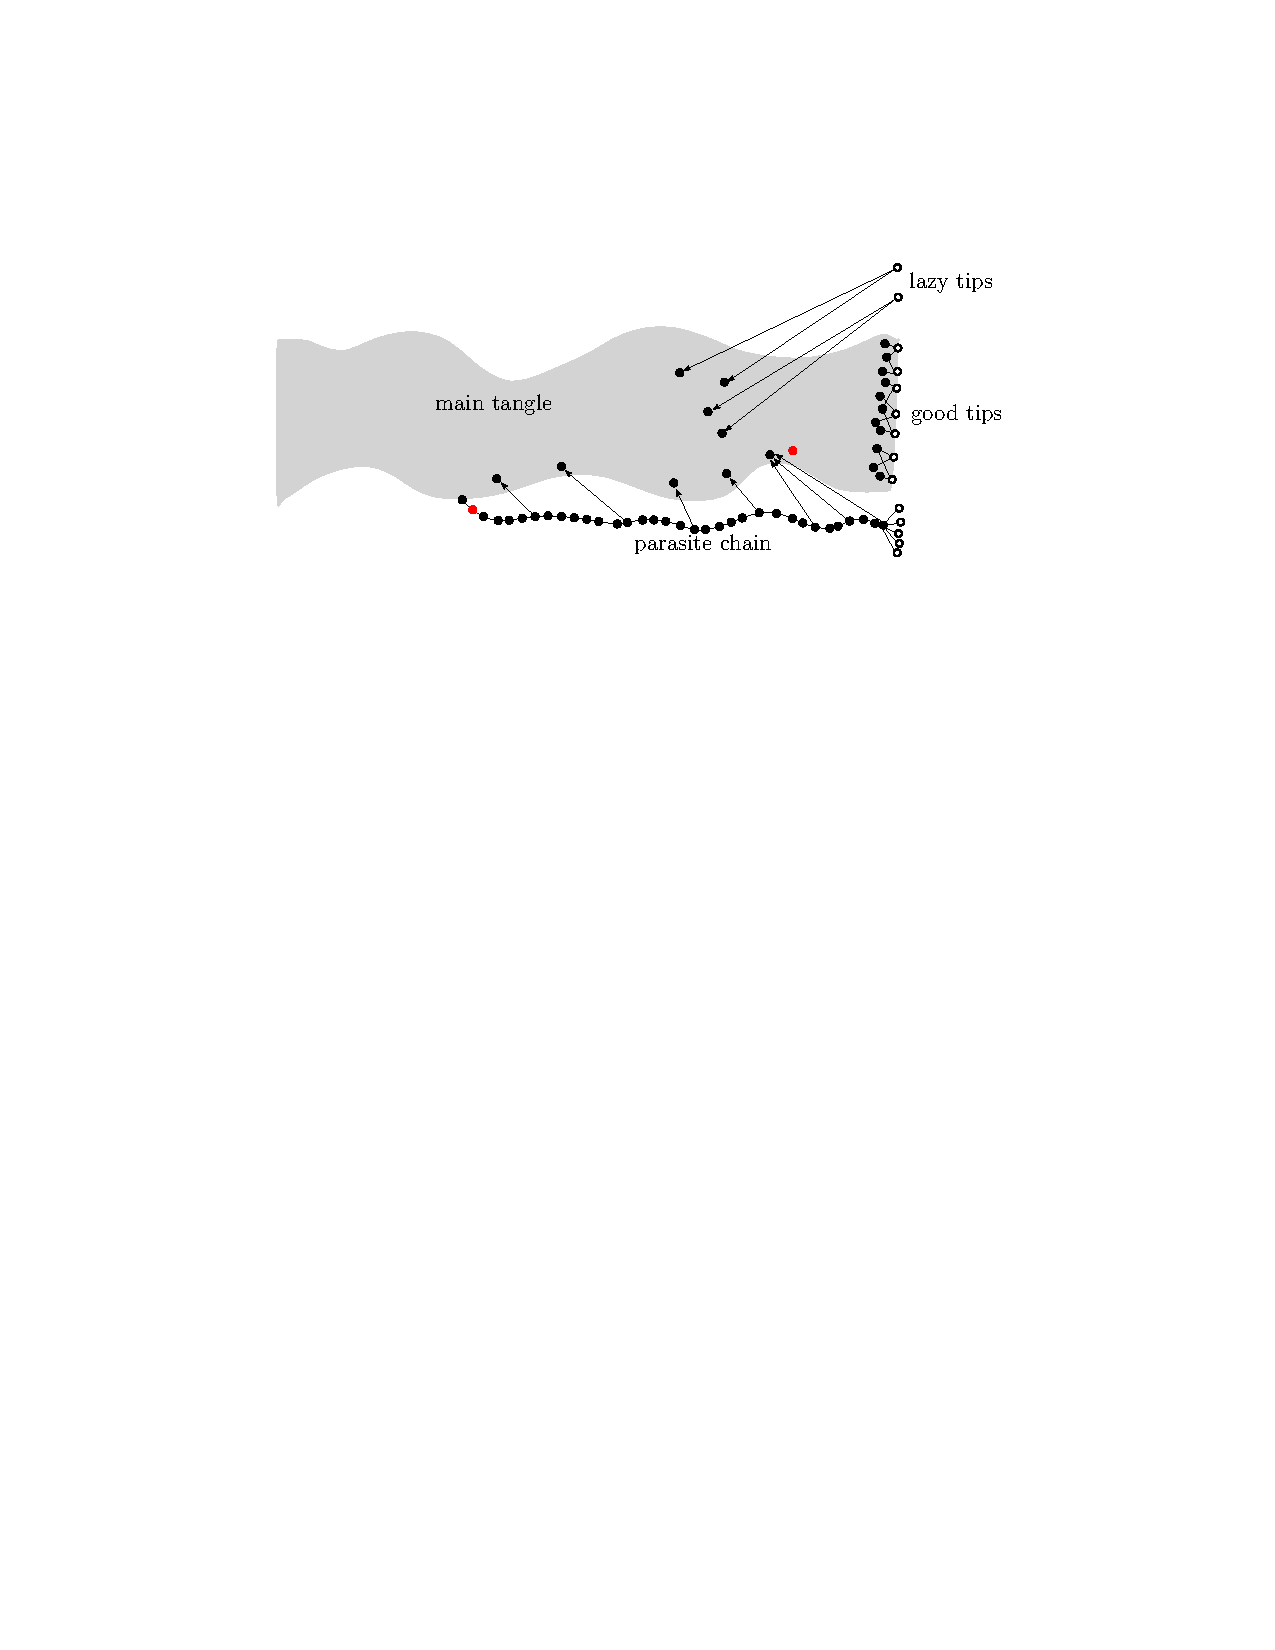
\includegraphics[width=12cm]{images/parasite-chain.pdf}
    \caption{Parasite Chain Attack \cite{the-tangle}}
    \label{fig:parasite-chain}
\end{figure}




